\section{Large Figures}\label{sec:app}

\subsection{Schematic of sensorboard}\label{app:schemmain}
%Image of schematic(s) (Rev 3)
\begin{figure}[h]
	\centering
    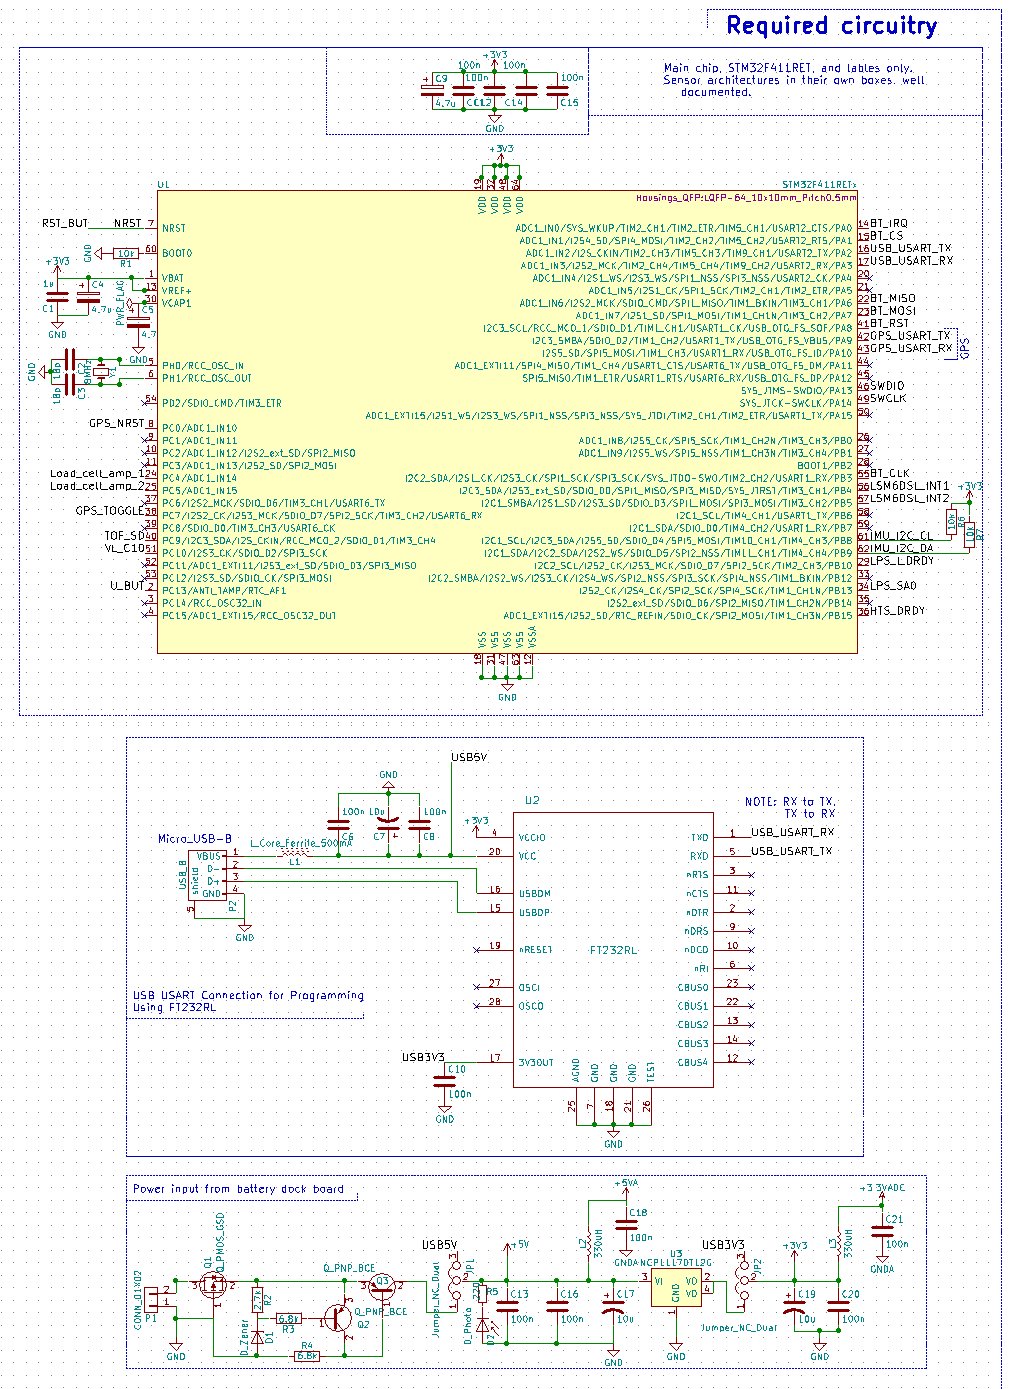
\includegraphics[width=.91\linewidth]{Figures/schem_r3_a.png}
	\captionsource{Schematic of revision 3, part a: Required circuitry.}{Author}
	\label{fig:schr3a}
\end{figure}
\begin{figure}[h]
	\centering
    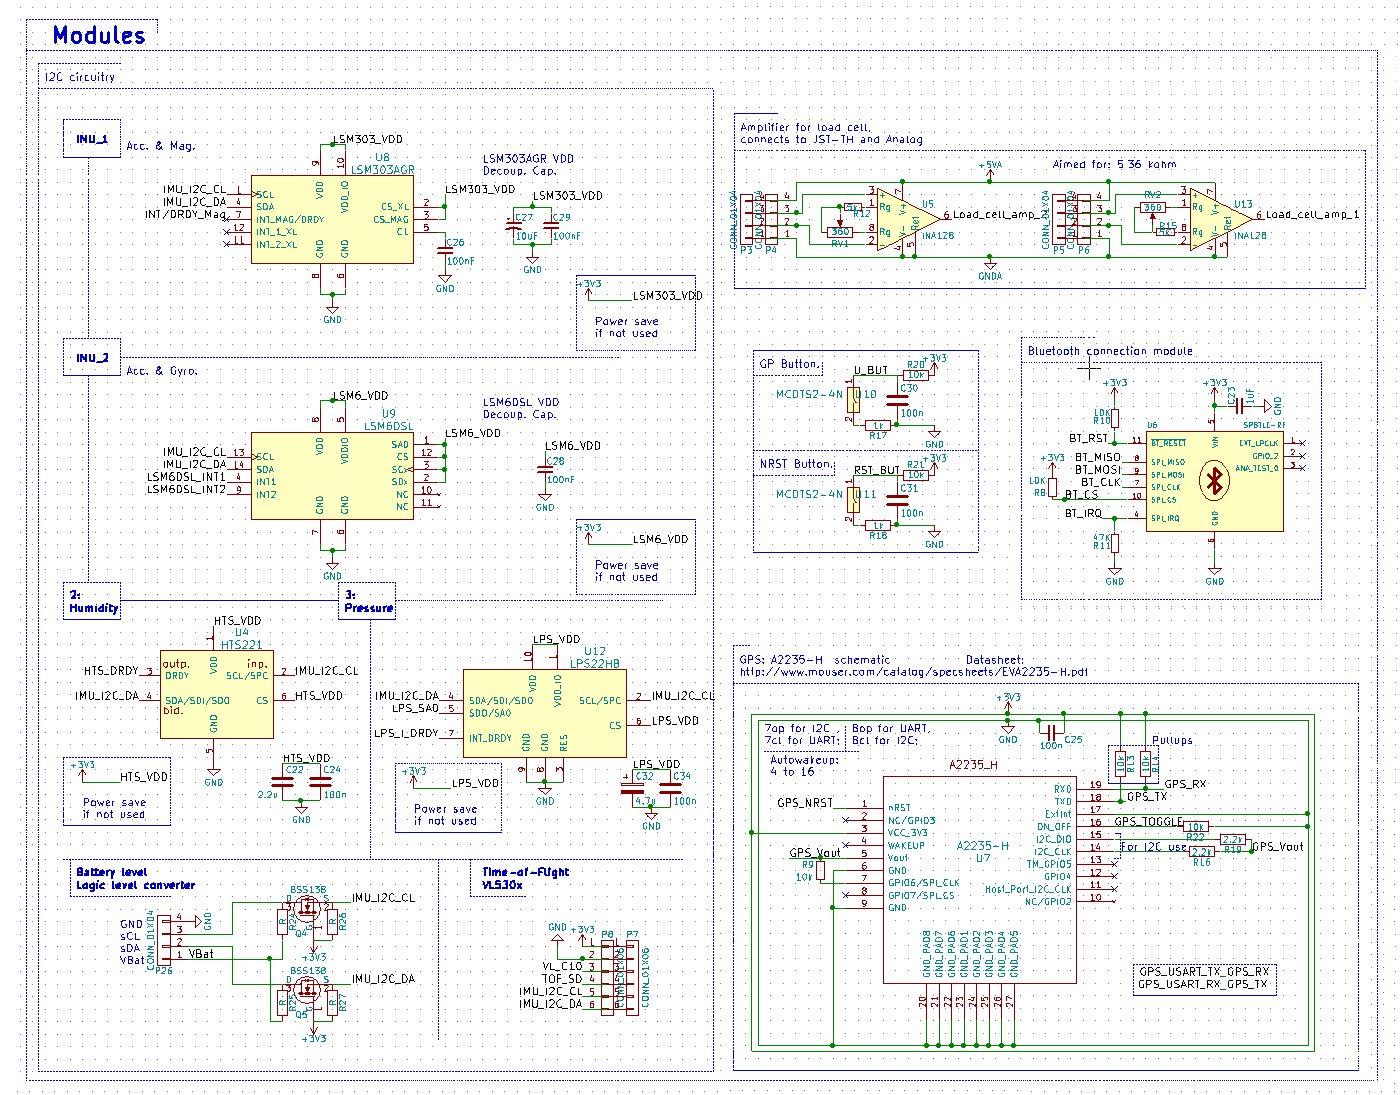
\includegraphics[width=\linewidth]{Figures/schem_r3_b.png}
	\captionsource{Schematic of revision 3, part b: Modules.}{Author}
	\label{fig:schr3b}
\end{figure}
\begin{figure}[h]
	\centering
    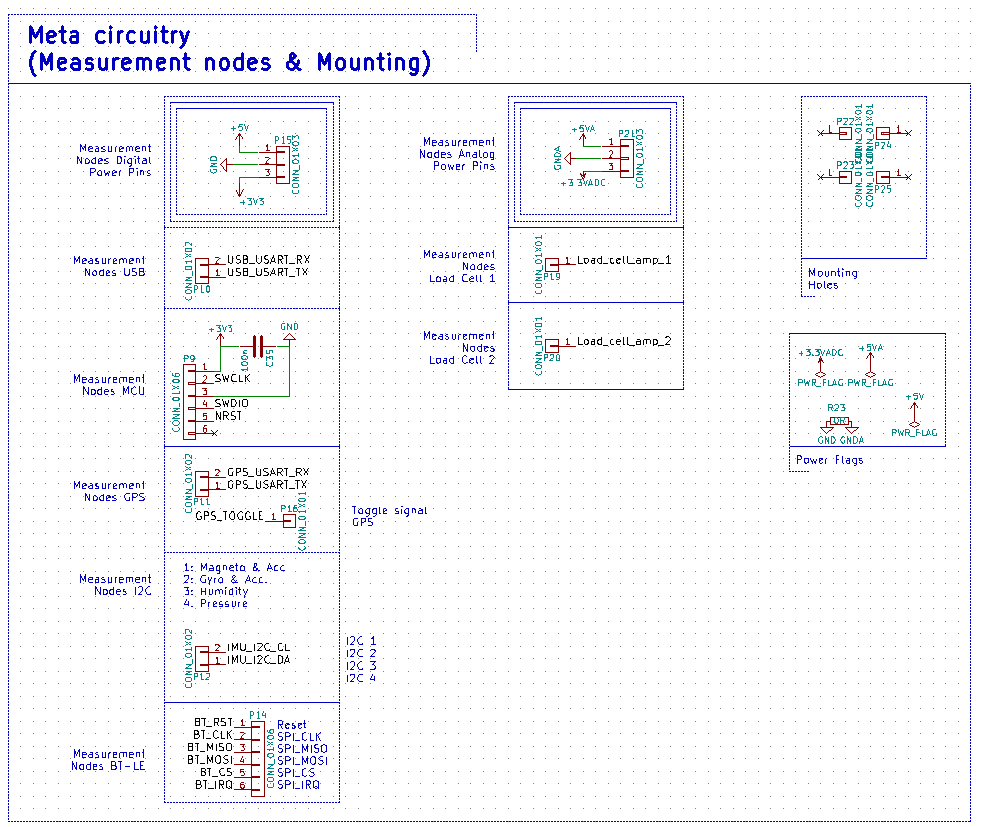
\includegraphics[width=\linewidth]{Figures/schem_r3_c.png}
	\captionsource{Schematic of revision 3, part c: Meta circuitry.}{Author}
	\label{fig:schr3c}
\end{figure}

\clearpage
\subsection{Schematic of \gls{bms}}\label{app:bms}
\begin{figure}[h]
	\centering
    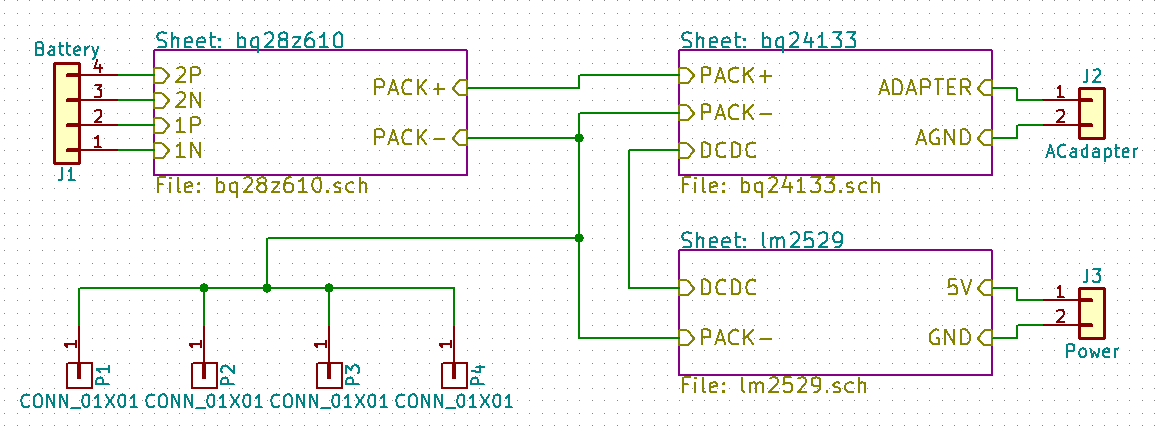
\includegraphics[width=.9\linewidth]{Figures/gasgauge_sch_root.png}
	\captionsource{Root schematic of \gls{bms} circuitry.}{Author}
	\label{fig:schbmsr}
\end{figure}
\begin{figure}[h]
	\centering
    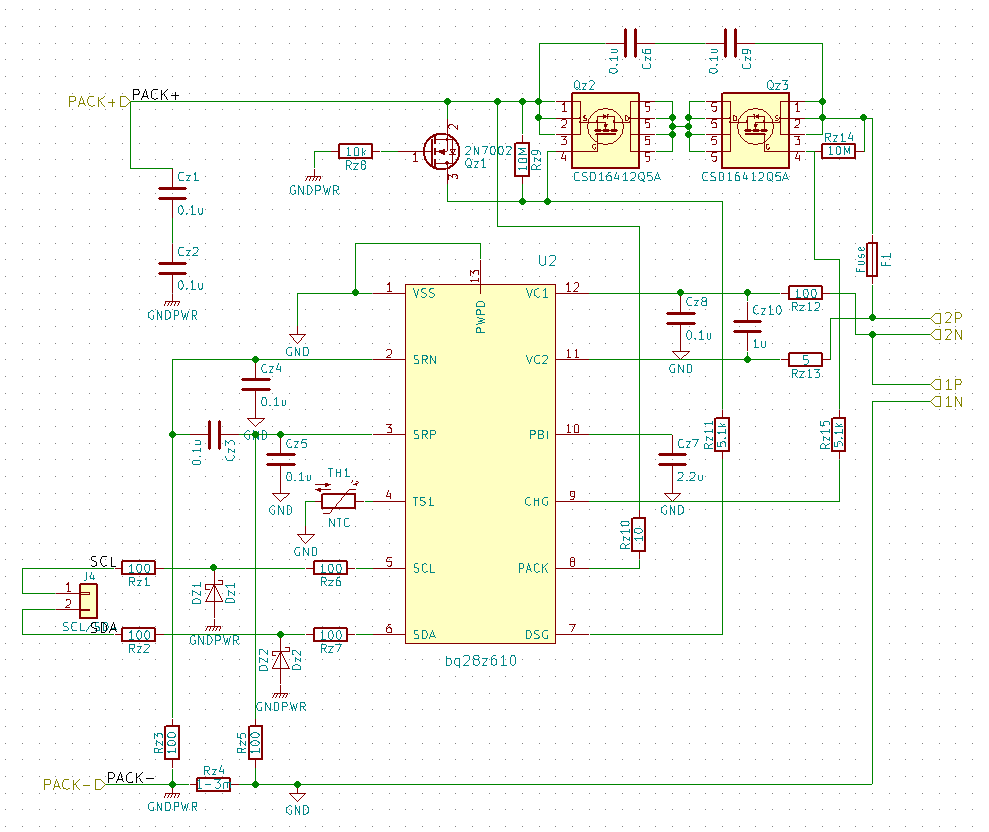
\includegraphics[width=.9\linewidth]{Figures/gasgauge_sch_bq28z610.png}
	\captionsource{Schematic of \gls{bms}, part a: bq28z610.}{Author}
	\label{fig:schbmsr}
\end{figure}
\begin{figure}[h]
	\centering
    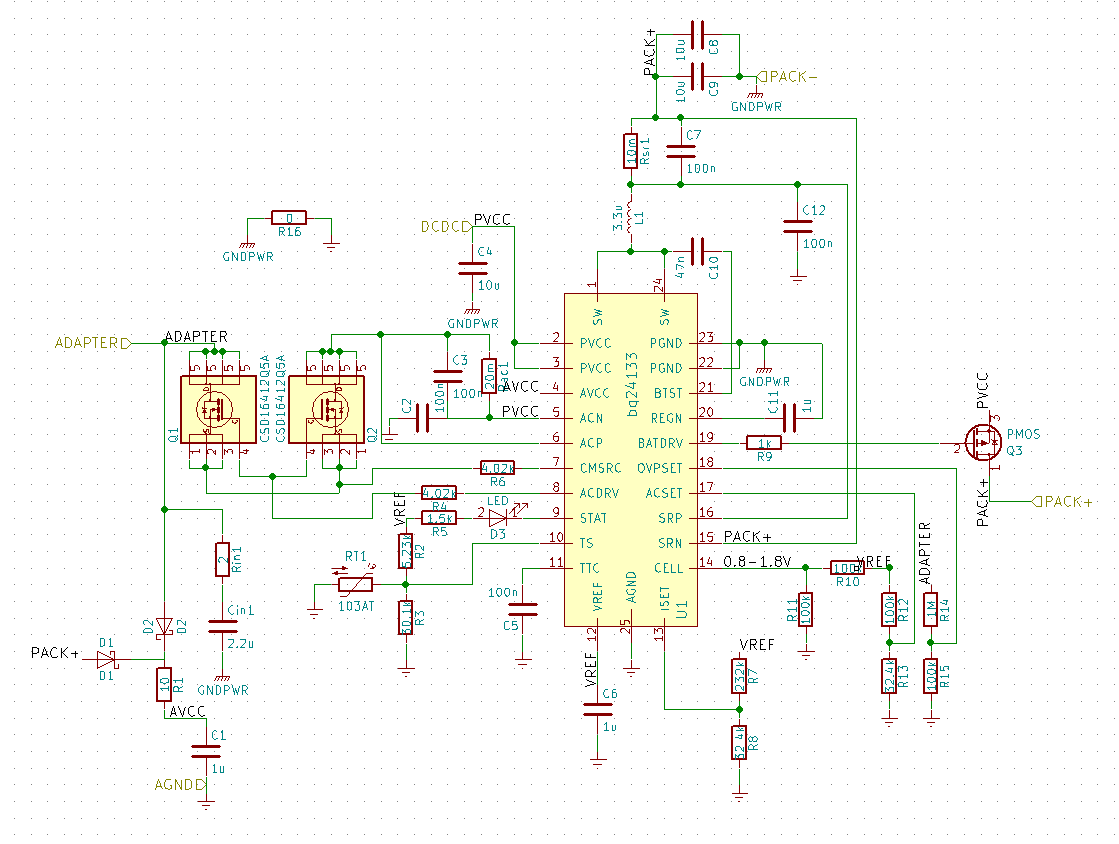
\includegraphics[width=\linewidth]{Figures/gasgauge_sch_bq24133.png}
	\captionsource{Schematic of \gls{bms}, part b: bq24133.}{Author}
	\label{fig:schbmsr}
\end{figure}
\begin{figure}[h]
	\centering
    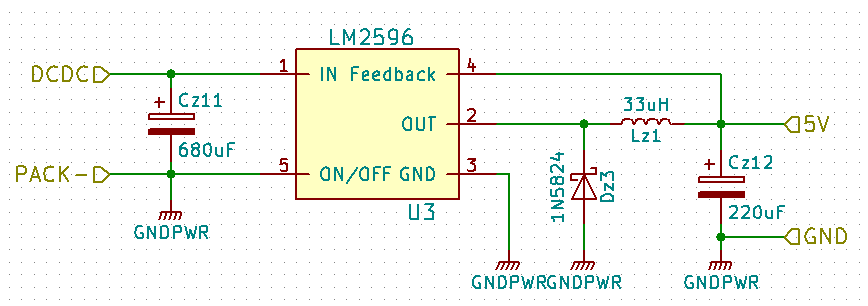
\includegraphics[width=\linewidth]{Figures/gasgauge_sch_lm2529.png}
	\captionsource{Schematic of \gls{bms}, part c: lm2596.}{Author}
	\label{fig:schbmsr}
\end{figure}


\clearpage
\subsection{CubeMX software}\label{sec:app:mxc}
% Image of CubeMX software
\begin{figure}[tbh]
	\centering
    	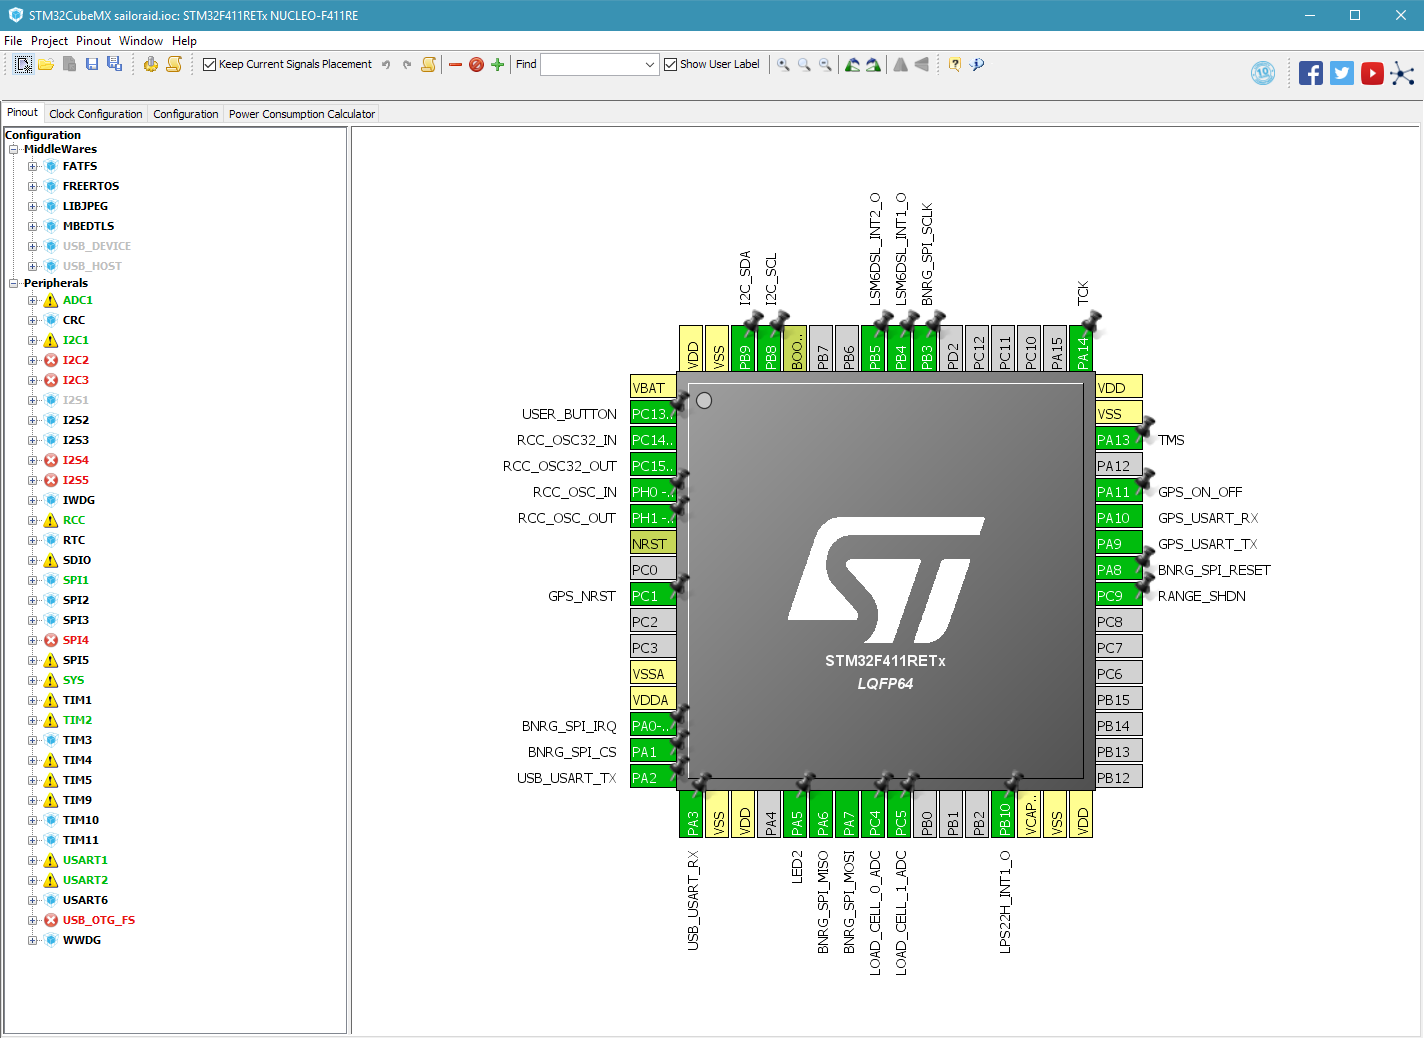
\includegraphics[width=\linewidth]{Figures/MXCube.png}
	\captionsource{CubeMX software}{Author}
	\label{fig:mxc}
\end{figure}

\clearpage
\section{Other Figures}
\subsection{Casing Dimensions}
\begin{figure}[htb]
	\centering
    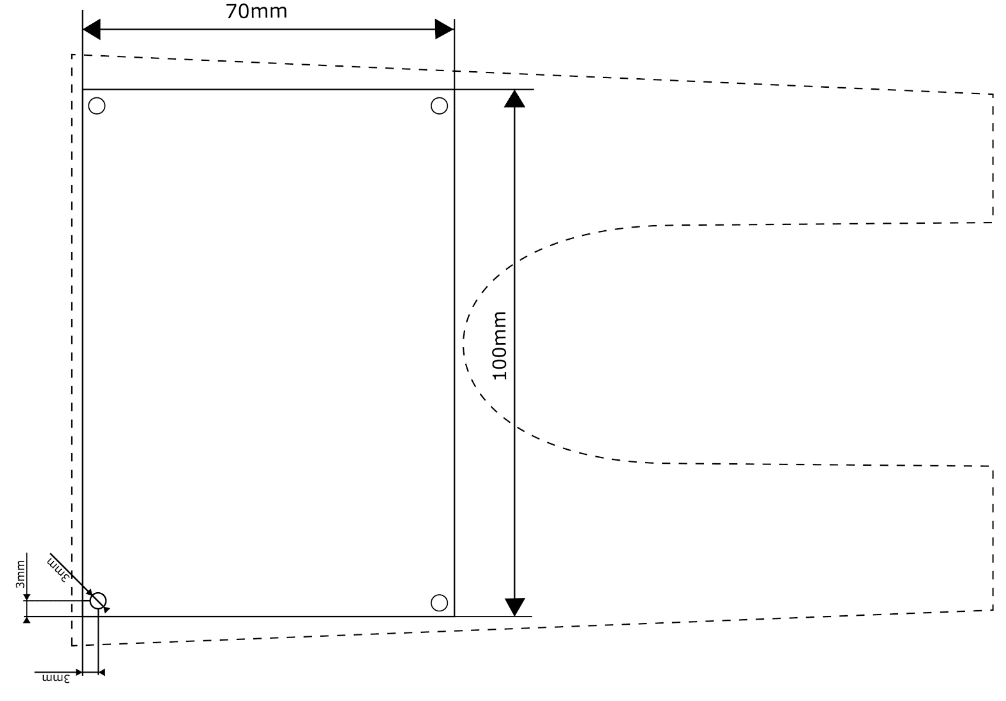
\includegraphics[width=\linewidth]{Figures/casing_dimensions.png}
	\captionsource{System enclosure shape and dimensions}{Author}
	\label{fig:casdim}
\end{figure}

\clearpage
\section{Lists}
\subsection{Bill of Materials: Main \gls{pcb}}
\begin{center}
\begin{tabular}{|l|l|c|}
	\hline
	\bf{Main Board Components} & \bf{Package} & \bf{Quantity} \\
	\hline
	\emph{Capacitors:} & & \\
	\hline
	18p & 0805 & 2 \\
	\hline
	100n & 0805 & 21 \\
	\hline
	1u & 0805 & 2 \\
	\hline 
	2.2u & 0805 & 1 \\
	\hline 
	4.7u & 0805 & 4 \\
	\hline 
	10u & Electrolytic SMD 5x5.3 & 6 \\
	\hline
	\emph{Resistors:} & & \\
	\hline
	220 & 0805 & 1 \\
	\hline
	1k & 0805 & 2 \\
	\hline
	1k & potentiometer & 2 \\
	\hline
	2.2k & 0805 & 2 \\
	\hline
	2.7k & 0805 & 1 \\
	\hline
	5k & 0805 & 2 \\
	\hline
	6.8k & 0805 & 2 \\
	\hline
	10k & 0805 & 11 \\
	\hline
	47k & 0805 & 1 \\
	\hline
	\emph{Inductors:} & & \\
	\hline
	1.5u & 1206 & 1 \\
	\hline 
	330u & Radial 200mil Pin Pitch & 2 \\
	\hline 
	\emph{Integrated Circuits:} & & \\
	\hline
	STM32F411RE & LPQF64 & 1 \\
	\hline 
	SPBTLE-RF & Custom & 1 \\
	\hline
	A2235-H & Custom & 1 \\
	\hline
	FT232R & SSOP-28 & 1 \\
	\hline
	LSM6DSL & LGA-14L & 1 \\
	\hline
	LSM303AGR & LGA-12 & 1 \\
	\hline
	HTS221 & HLGA-6L & 1 \\
	\hline
	LPS22HB & HLGA-10L & 1 \\
	\hline
	INA128 & SOIC-8 & 2 \\
	\hline
	LM1117-3.3 & SOT-223 & 1 \\
	\hline
	\emph{Semiconductors:} & & \\
	\hline
	P-MOS PMV65XP & SOT-23 & 1 \\
	\hline
	PNP BJT FMMT718 & SOT-23 & 2 \\
	\hline
	Zener Diode, 5.6V & SOD-323 & 1 \\
	\hline
	Green LED & ø2.5mm 100mil pitch& 1 \\
	\hline
	\emph{Others:} & & \\
	\hline
	Tactile SMD Button & & 2 \\
	\hline
	8MHz Crystal & & 1 \\
	\hline
	Micro USB-B & & 1 \\
	\hline
	Straight 6-Pin Header & 100mil pitch & 1 \\
	\hline
	Straight 3-Pin Header & 100mil pitch & 2 \\
	\hline
	Pin Jumper & & 2 \\
	\hline
\end{tabular}
\end{center}

\clearpage
\subsection{Bill of Materials: Battery Management \gls{pcb}}
%\begin{center}
\begin{tabular}{|l|l|c|}
	\hline
	\bf{Battery Management Circuit} & \bf{Package} & \bf{Quantity} \\
	\hline
	\emph{Capacitors:} & & \\
	\hline
	47n & 0603 & 1 \\
	\hline
	100n & 0603 & 13 \\
	\hline
	1u & 0603 & 4 \\
	\hline
	2.2u & 0603 & 2 \\
	\hline
	10u & 1206 & 3 \\
	\hline
	220u & Electrolytic SMD 6.3x5.8 & 1 \\
	\hline
	680u & Electrolytic SMD 6.3x5.8 & 1 \\
	\hline
	\emph{Resistors:} & & \\
	\hline
	0 & 0603 & 1 \\
	\hline
	1-3m & 2512 & 1 \\
	\hline
	10m & 2512 & 1 \\
	\hline
	20m & 2512 & 1 \\
	\hline
	2 & 2010 & 1 \\
	\hline
	5 & 2512 & 1 \\
	\hline
	10 & 0603 & 1 \\
	\hline
	10 & 1206 & 1 \\
	\hline
	100 & 0603 & 7 \\
	\hline
	100 & 2512 & 1 \\
	\hline
	1k & 0603 & 1 \\
	\hline
	1.5k & 0603 & 1 \\
	\hline
	4.02k & 0603 & 2 \\
	\hline
	5.1k & 0603 & 2 \\
	\hline
	5.23k & 0603 & 1 \\
	\hline
	10k & 0603 & 1 \\
	\hline
	30.1k & 0603 & 1 \\
	\hline
	32.4k & 0603 & 2 \\
	\hline
	100k & 0603 & 4 \\
	\hline
	232k & 0603 & 1 \\
	\hline
	1M & 0603 & 1 \\
	\hline
	10M & 0603 & 2 \\
	\hline
	103AT & Axial Standing 100mil Pitch & 2 \\
	\hline 
	\emph{Inductors:} & & \\
	\hline
	3.3u & 7.3x7.3mm SMD & 1 \\
	\hline
	33u & 12x12mm SMD & 1 \\
	\hline
	\emph{Integrated Circuits:} & & \\
	\hline
	BQ24133 & VFQN-24 & 1 \\
	\hline
	BQ28Z610 & S-PDSO-N12 & 1 \\
	\hline
	LM2529 & TO-263-5 & 1 \\
	\hline
	\emph{Semiconductors:} & & \\
	\hline
	Schottky Diode & SOD-323 & 4 \\
	\hline
	1N5824 & Axial 10.16mm Pitch & 1 \\
	\hline
	N-MOS CSD16412Q5A & TDSON-8-1 & 4 \\
	\hline
	Red LED & ø3mm Radial 100mil Pitch & 1 \\
	\hline
	2N7002 & SOT-23 & 1 \\
	\hline
	Power P-MOS & SOT-23 & 1 \\
	\hline
\end{tabular}
%\end{center}
%Image of circuit board(s) are sectionlocals labled as "fig:pcbr*"
%Local. Image of casing
%INSERT Image of complete/mounted system